\documentclass[class=NTHU_thesis, crop=false]{standalone}
\begin{document}

\chapter{The MonoH Analysis}
\section{Background Estimation Strategy}
The main background processes of the analysis are $Z$($\nu\nu$) + jets, $W$($l\nu$) + jets and $t\bar{t}$, shown in Figure \ref{fig:Bkg-Processes}. In the $Z$($\nu\nu$) + jets process, the undetectable neutrinos in the final state are regarded as the missing energy. Thus once the jets are tagged as $b$-jets, the case will be background. In the $W$($l\nu$) + jets process, once the lepton is misidentified as the missing energy and the jets are tagged as $b$-jets as mentioned previously, the procedure will be interference as well. In the $t\bar{t}$ case, if both the leptons are misidentified, the process will be background.

\begin{figure}[!hbt]
	\captionsetup[subfigure]{labelformat=empty}
	\centering
	\subcaptionbox
	{$Z$($\nu\nu$) + jets
		\label{fig:Bkg-Processes-fig1}}
	{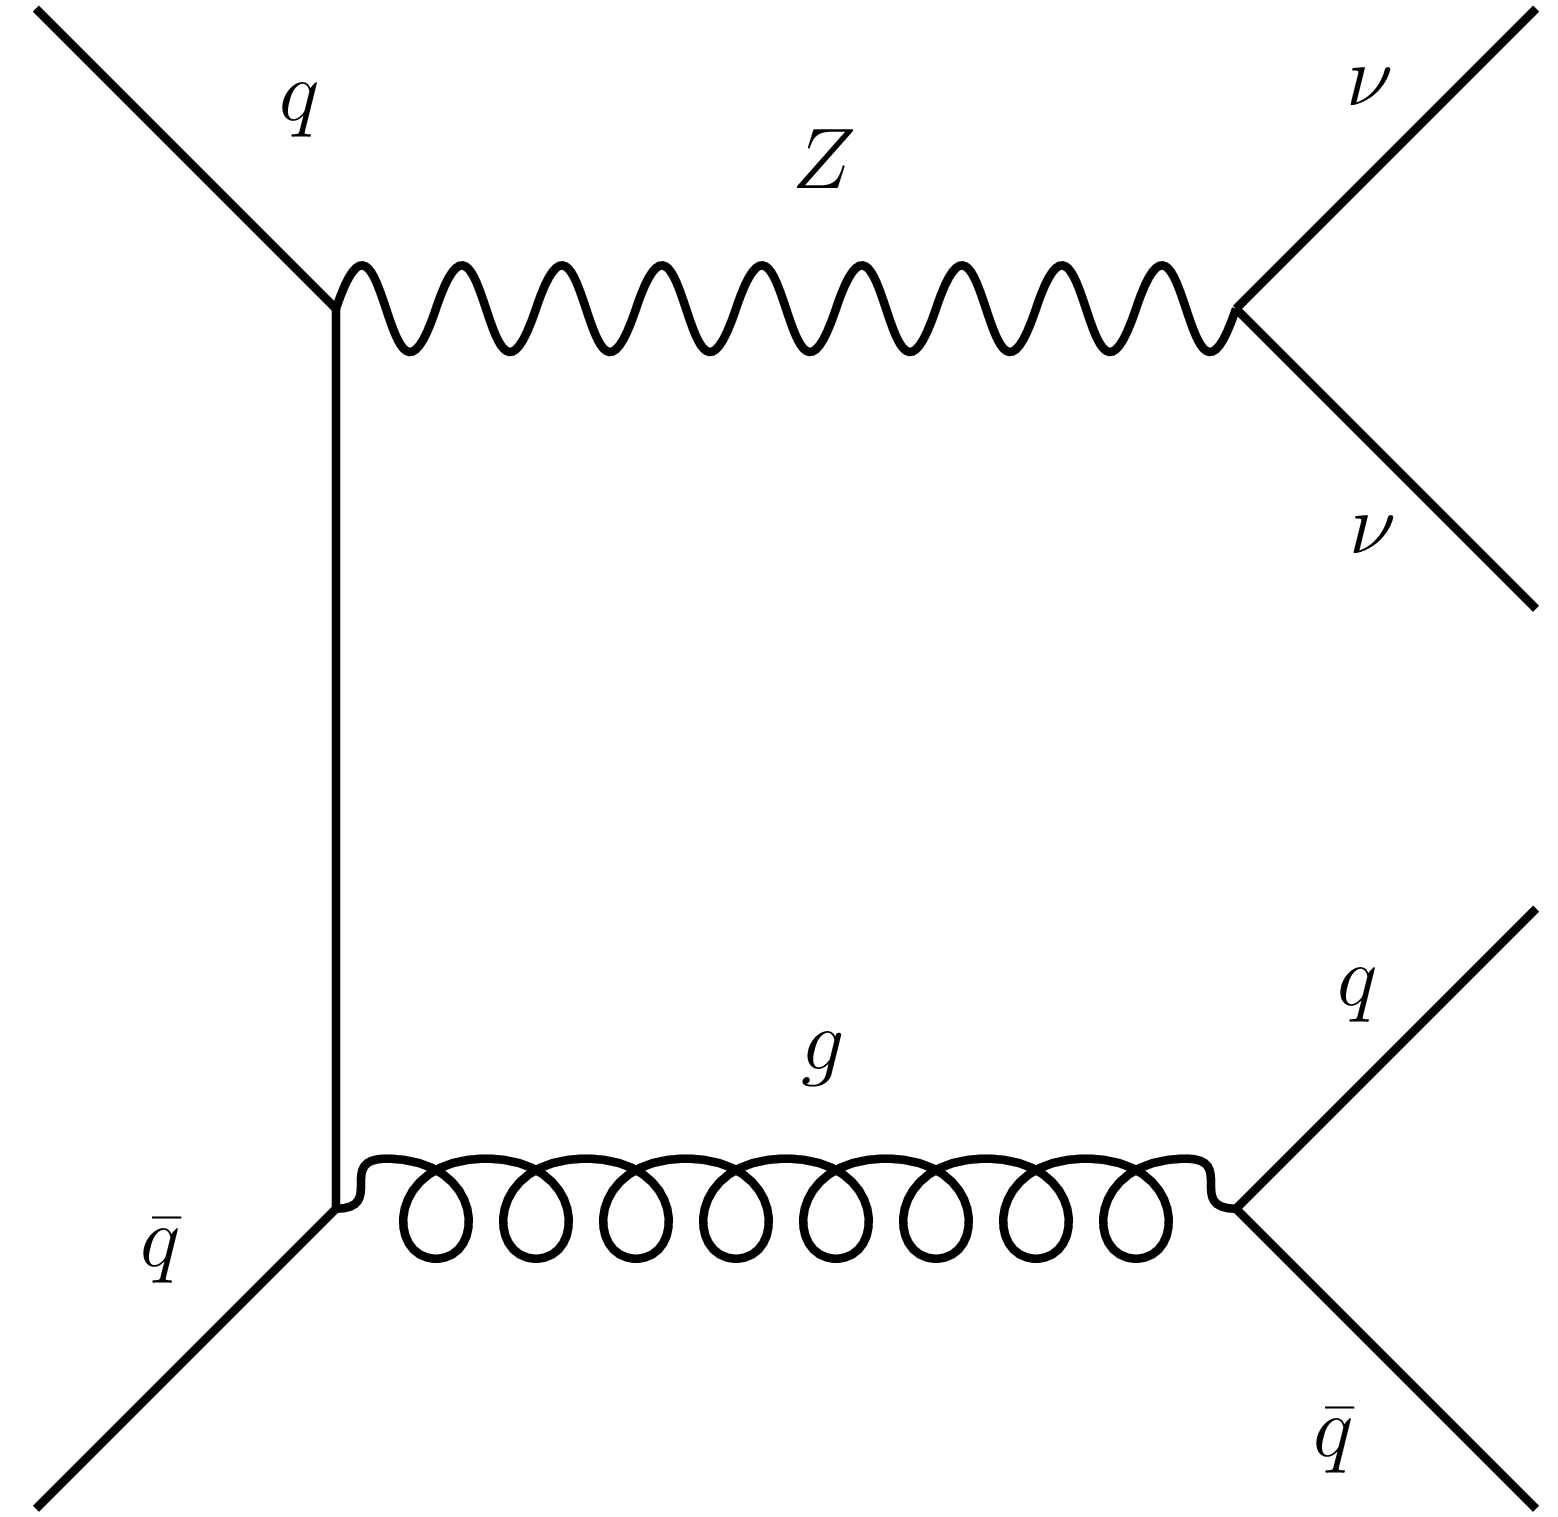
\includegraphics[width=0.3\linewidth]{Zvv.png}}
	~
	\subcaptionbox
	{$W$($l\nu$) + jets
		\label{fig:Bkg-Processes-fig2}}
	{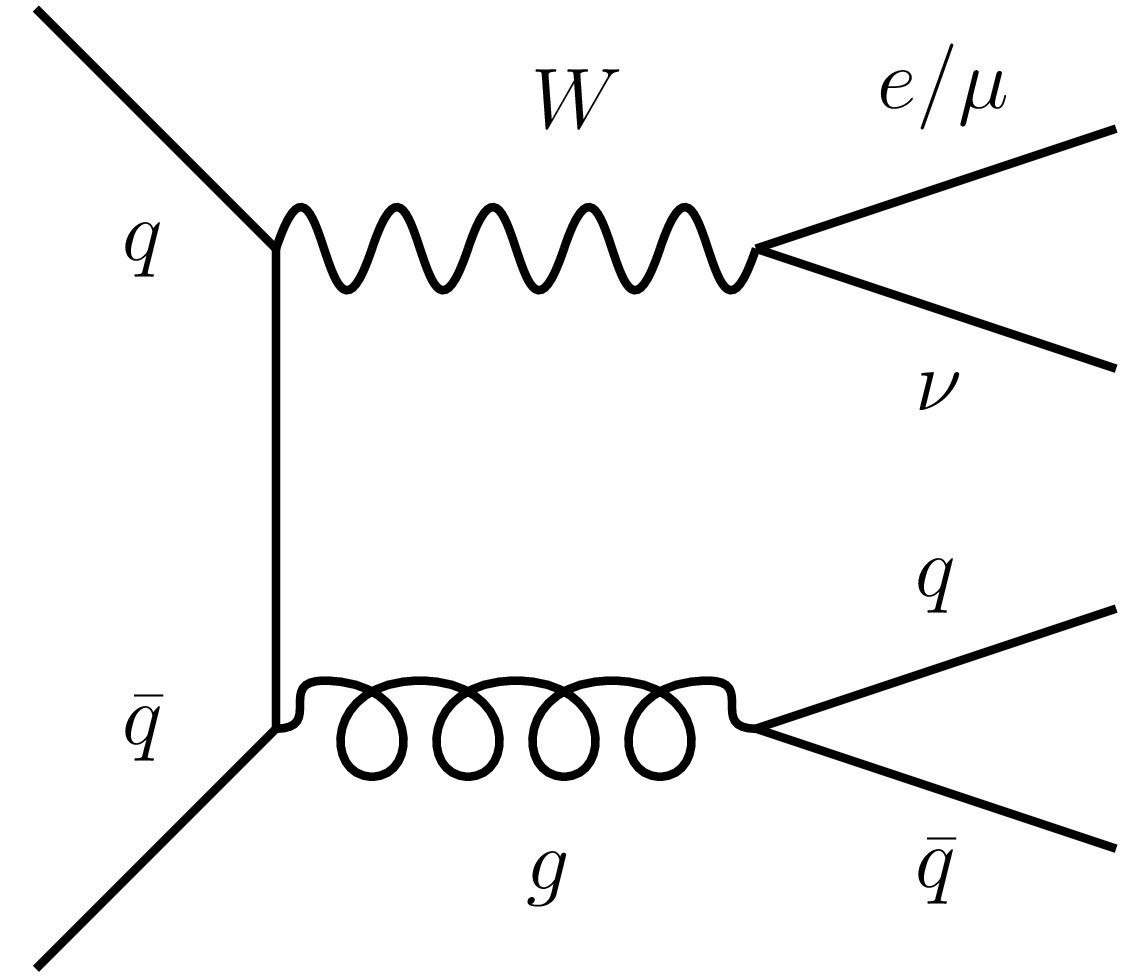
\includegraphics[width=0.3\linewidth]{Wlv.png}}
	~
	\subcaptionbox
	{$t\bar{t}$
		\label{fig:Bkg-Processes-fig3}}
	{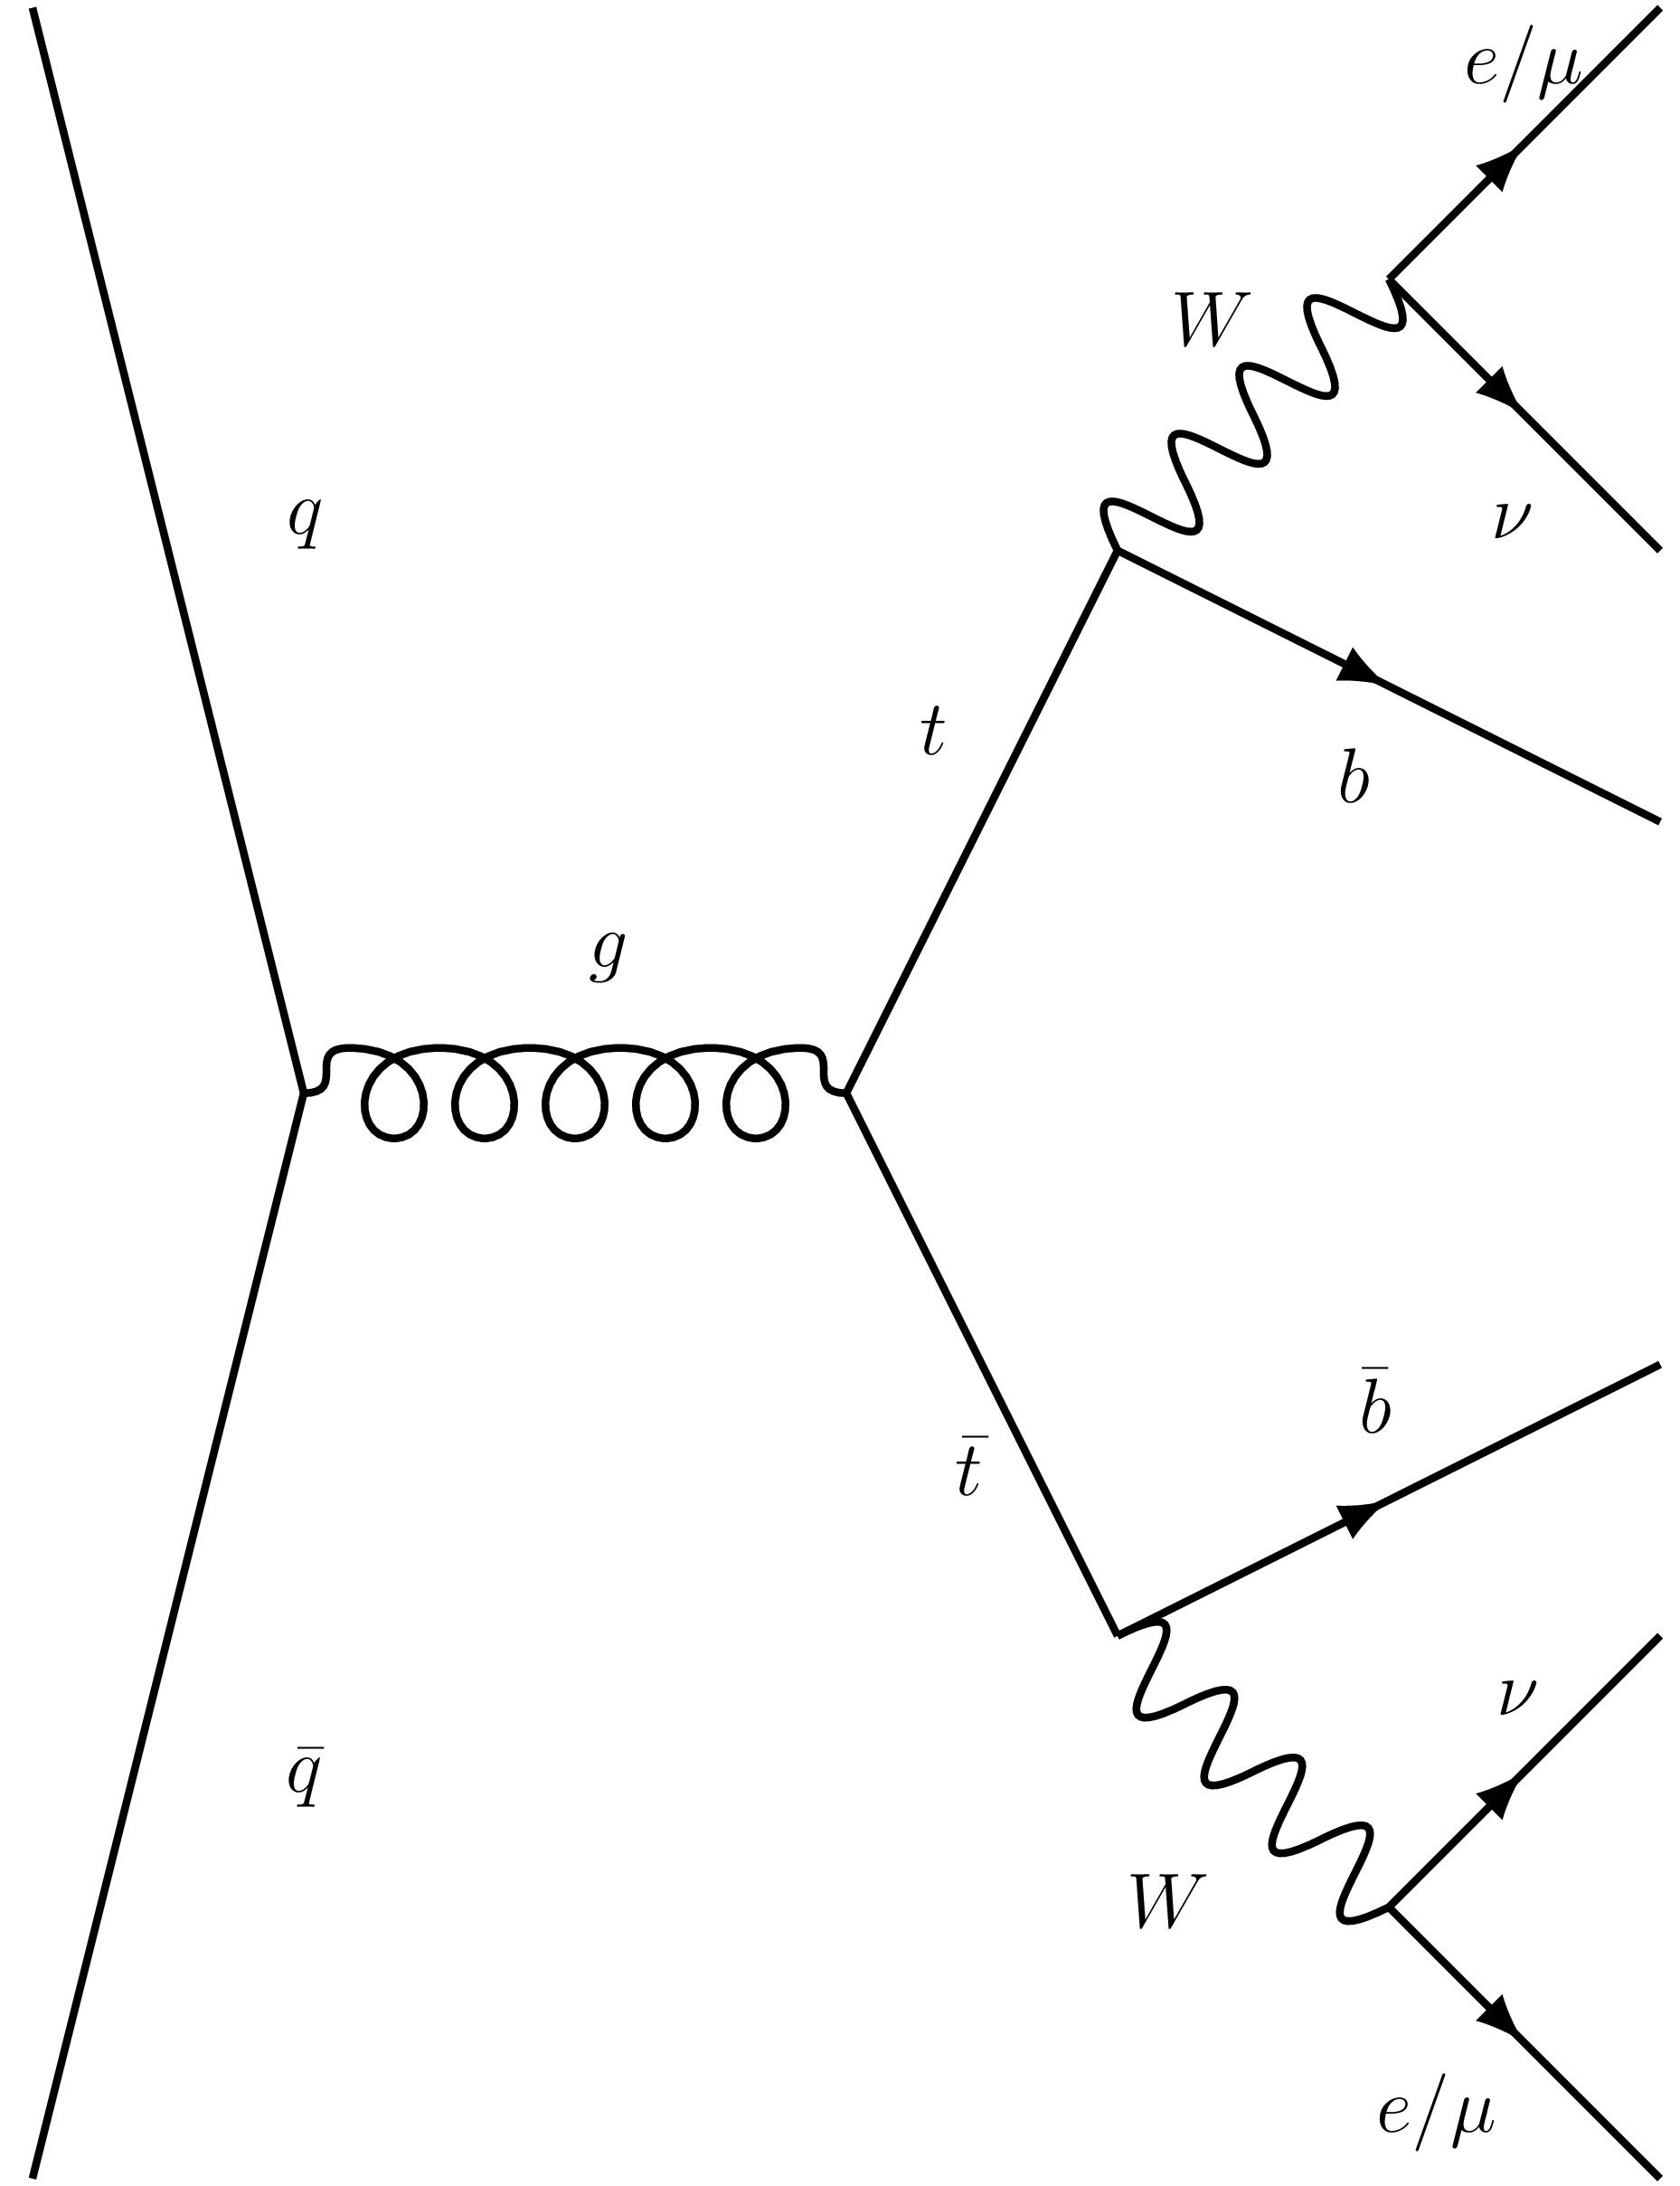
\includegraphics[width=0.3\linewidth]{ttbar.png}}
	\caption{The main background processes of the monoH analysis.}
	\label{fig:Bkg-Processes}
\end{figure}

To constrain these background, the control region (CR) strategy is used. Before defining the CR, the signal region (SR) is defined as where the signals are expected to show. The SR is required to have no lepton based on the model. Then the CR is defined as the orthogonal region to the SR. Exploiting the similar kinematics, the CRs use some better-measured processes in order to constrain the background. There are two CRs in this analysis, the one-muon CR and the two-lepton CR. The one-muon CR contains two processes, $W$($\mu\nu$) + jets and $t\bar{t}$, constraining $W$($l\nu$) + jets and $t\bar{t}$ in the SR. It requires different number of misidentified leptons, for $W$($l\nu$) + jets, one misidentified lepton in the SR but none in the one-muon CR, and for $t\bar{t}$, two misidentified leptons in the SR but one in the one-muon CR. The two-lepton CR exploits the $Z$($ll$) + jets, constraining the $Z$($\nu\nu$) + jets process.

\section{Object Reconstruction and Selection}
\subsection{Jets}
Jets are a method to describe hadronic showers in detectors, consisting of multiple objects. Jets are reconstructed with the anti-$k_t$ algorithm\cite{1126-6708-2008-04-063}. Depending on the toplogical clusters, the radius parameter of $R = 0.4$ is the small-radius (small-$R$) jets and of $R = 1.0$ is the large-radius (large-$R$) jets.

The small-$R$ jets with $p_T > 20\, \mathrm{GeV}$ for $\left|\eta\right| < 2.5$ are regarded to as the central jets. The MV2c10 discriminant is used for $b$-tagging the central jets to identify the $b$-hadrons, with the 77\% efficiency working point. In addition, the small-$R$ jets with $p_T > 30\, \mathrm{GeV}$ for $2.5 < \left|\eta\right| < 4.5$ are the forward jets. The large-$R$ jets are required to have $p_T > 200\, \mathrm{GeV}$ and $\left|\eta\right| < 2.0$, containing multiple constituent jets called the track jets. The flavor identification for the large-$R$ jets depend on the ghost-associated track jets with the MV2c10 discriminant with the 77\% $b$-tagging efficiency working point. The track jets are described more in the following.

The fixed-radius (FR) track jets are applied for $b$-tagging in the previous analysis, using the anti-$k_t$ algorithm with fixed radius parameters. Instead of the FR track jets, the variable-radius (VR) track jets are implemented in the analysis for improving the $b$-tagging efficiency. The primary characteristic of the VR track jets is the relevance between the $p_T$ and the jet radius parameter: 
\begin{equation}
R \to R_{eff}(p_T) \approx \frac{\rho}{p_T}
\end{equation}
where $\rho$ is a constant factor.

\subsection{Leptons}
Electrons are reconstructed with energy deposits in the EM calorimeter which matches tracks in the ID. Besides the basic reconstruction, there are two types of electrons for the further selection in the analysis, the baseline electrons and the signal electrons. The baseline electrons have a loose criterion with $\left|\eta\right| < 2.47$ and $p_T > 7\, \mathrm{GeV}$, used for electron vetoes. For the events containing electrons, the signal electrons require $\left|\eta\right| < 2.47$ and $p_T > 27\, \mathrm{GeV}$.

The muon reconstruction relies on the muon spectrometer in the range of $\left|\eta\right| < 2.7$. It's also claimed to match the tracks in the ID for $\left|\eta\right| < 2.5$. Like electrons, there are two categories of muons, the baseline muons and the signal muons. The baseline muons are used for vetoing events in certain regions, requiring $\left|\eta\right| > 2.7$ and $p_T < 7\, \mathrm{GeV}$. The signal muons are defined with the criterion of $\left|\eta\right| < 2.5$ and $p_T > 25\, \mathrm{GeV}$ for the events which contain muons.

Because of the hadronic-like nature of taus, the reconstruction is complicated and described in \cite{ATLAS-CONF-2017-029}. For the tau vetoes in the analysis, the taus are required to have one or three tracks and have $\left|\eta\right| < 2.5$ and $p_T > 20\, \mathrm{GeV}$, excluding the crack region $1.37 < \left|\eta\right| < 1.52$.

\subsection{Missing Transverse Momentum}
The missing transverse momentum is determined as the negative vector sum of the transverse momentum of all the reconstructed and calibrated objects in an event. Additionally, the track-based soft term is added into the missing transverse momentum in the analysis, which is from the tracks that not associated with any reconstructed object but still linked to the primary vertex. The absolute value of the missing transverse momentum is expressed as $E^{miss}_T$. Also, there is a purely track-based missing transverse momentum calculated as the negative vector sum of the transverse momentum of all the reconstructed tracks associated with the primary vertex. The absolute value of the track-based missing transverse momentum is denoted as $p^{miss}_T$.

Furthermore, to recognize whether the $E^{miss}_T$ is from weakly interacting particles or from the mis-measurement of multi-jet processes, two kinds of the $E^{miss}_T$ significance are applied. One is the event-based $E^{miss}_T$ significance which is performed in previous monoHbb analysis, and the other is the object-based $E^{miss}_T$ significance which is newly introduced in the analysis. The object-based $E^{miss}_T$ significance is defined in \cite{ATLAS-CONF-2018-038}.

\section{Event Selection}
All the event data are from the proton-proton collision at $\sqrt{s} = 13 TeV$, recorded by the ATLAS detector during 2015, 2016 and 2017. Only data passed good operating conditions are used for the data quality. The integrated luminosity is $79.8 \pm 1.6 fb^{-1}$ in the analysis.

To meet the lepton conditions of the SR and the CRs, the events with no lepton, with exactly one signal muon, and with exactly two baseline leptons of which at least one is a signal lepton, are respectively accepted in SR, one-muon CR and two-lepton CR. The SR is divided into two parts, the resolved region ($E^{miss}_T < 500\, \mathrm{GeV}$) and the merged region ($E^{miss}_T > 500\, \mathrm{GeV}$), for different event selection requirements. As previously mentioned in 3.1, to be the comparison of the SR, the CRs are also divided into two divisions with the $p_T$ of the vector boson ($W$ or $Z$) as the separation boundary ($p^V_T < 500\, \mathrm{GeV}$ for the resolved region and $p^V_T > 500\, \mathrm{GeV}$ for the merged region). The total event selection is summarized in Table \ref{table:summary_event_selection}.

The events are required to be done some common selections in both the resolved and merged regions. They have to pass the lowest un-prescaled triggers, and have at least one reconstructed vertex with at least two associated tracks with $p_T > 0.4\, \mathrm{GeV}$. To suppress the non-collision processes, the events are selected if $E^{miss}_T > 150\, \mathrm{GeV}$ in the SR and $p^V_T > 150\, \mathrm{GeV}$ in the CRs. Also, the events with tau leptons are vetoed. Moreover, in order to reduce the multi-jet processes, two conditions are applied. First, the azimuthal angular difference between $E^{miss}_T$ and the three highest small-$R$ jets (min$\Delta\phi(E^{miss}_T, jets_{1, 2, 3})$) is required to be larger than $20^\circ$. Second, the azimuthal angular difference between the direction of $E^{miss}_T$ and $p^{miss}_T$ ($\Delta\phi(E^{miss}_T, p^{miss}_T)$) is required to less than $90^\circ$. In addition, $H_T$ ratio cut is performed to reduce the $t\bar{t}$ background, which is referred in \cite{Meehan:2225941}.

In the resolved region, there are at least two central small-$R$ jets in the events. Exactly two of the jets are $b$-tagged and at least one of them have $p_T > 45\, \mathrm{GeV}$. The two $b$-tagged jets consist the Higgs boson candidate and their mass is required to be $50\, \mathrm{GeV} < m_{jj} < 280\, \mathrm{GeV}$. The scalar $p_T$ sum of first two (three) jets has to larger than $120 (150)\, \mathrm{GeV}$ for the events with two (three or more) jets. To further suppress the multi-jet background, the azimuthal difference between the Higgs boson candidate and $E^{miss}_T$ ($\Delta\phi(E^{miss}_T, h)$) is required to be larger than $120^\circ$. The azimuthal difference between the two jets which form the Higgs boson candidate ($\Delta\phi(jet_1, jet_2)$) is required to be less than $140^\circ$, and the ${\Delta}R$ between them to be less than $1.8$. In the SR and the one-muon CR, the object-based $E^{miss}_T$ significance is applied to be larger than $16$. Otherwise, the event-based $E^{miss}_T$ significance is applied to be less than $3.5$ in the two-lepton CR. The event-based $E^{miss}_T$ significance is defined as $E^{miss}_T/\sqrt{{\sum}p^l_T+{\sum}p^{jet}_T}$.

In the merged region, it is required that to have at least one central large-$R$ jet of which the leading one is associated with two leading $b$-tagged VR track jets. The events with any $b$-tagged VR track jet outside the large-$R$ jet are vetoed. The large-$R$ jet is the Higgs boson candidate and the mass is required to be $50 < m_{J} < 270\, \mathrm{GeV}$.

\begin{table}[!h]
	\centering
	\begin{tabularx}{1\textwidth}{ |
			>{\setlength\hsize{1\hsize}\centering}X|>{\setlength\hsize{1\hsize}\centering}X| } 
		\hline
		Resolved Region  & Merged Region \tabularnewline
		\hline \hline
		\multicolumn{2}{|c|}{number of leptons = 0 (SR), 1 (one-muon CR), 2 (two-lepton CR)} \tabularnewline
		\hline
		\multicolumn{2}{|c|}{lowest un-prescaled triggers, vertex requirement} \tabularnewline
		\hline
		$150\, \mathrm{GeV} < E^{miss}_T$ (SR), $p^V_T$ (CRs) $ < 500\, \mathrm{GeV}$ & $E^{miss}_T$ (SR), $p^V_T$ (CRs) $ > 500\, \mathrm{GeV}$ \tabularnewline
		\hline
		\multicolumn{2}{|c|}{$\tau$-veto} \tabularnewline
		\hline
		\multicolumn{2}{|c|}{min$\Delta\phi(E^{miss}_T, jets_{1, 2, 3}) > 20^\circ$} \tabularnewline
		\hline
		\multicolumn{2}{|c|}{$\Delta\phi(E^{miss}_T, p^{miss}_T) < 90^\circ$} \tabularnewline
		\hline
		\multicolumn{2}{|c|}{$H_T$ ratio cut} \tabularnewline
		\hline
		number of central small-$R$ jets = 2 & number of central large-$R$ jets = 1 \tabularnewline
		\hline
		$p^{jet_1}_T > 45\, \mathrm{GeV} \parallel p^{jet_2}_T > 45\, \mathrm{GeV}$ & - \tabularnewline
		 \hline
		2 $b$-tagged small-$R$ jets & 2 $b$-tagged VR track jets \tabularnewline
		\hline
		$50\, \mathrm{GeV} < m_{jj} < 280\, \mathrm{GeV}$ & $50\, \mathrm{GeV} < m_{J} < 270\, \mathrm{GeV}$ \tabularnewline
		\hline
		$\sum_{i = 1}^{2(3)} p^{jet_i}_T > 120 (150)\, \mathrm{GeV}$ & - \tabularnewline
		\hline
		$\Delta\phi(E^{miss}_T, h) > 120^\circ$ & - \tabularnewline
		\hline
		$\Delta\phi(jet_1, jet_2) < 140^\circ$& - \tabularnewline
		\hline
		${\Delta}R < 1.8$ & - \tabularnewline
		\hline
		$E^{miss}_T$ significance cut& - \tabularnewline
		\hline
	\end{tabularx}
	\caption{The summary of the event selection.}
	\label{table:summary_event_selection}
\end{table}

\section{Results of the MonoH Analysis}
The binned likelihood approach is used to get the final fitting result. The data are binned into four regions, three for the resolved region, $[150\, \mathrm{GeV}, 200\, \mathrm{GeV})$, $[200\, \mathrm{GeV}, 350\, \mathrm{GeV})$ and $[350\, \mathrm{GeV}, 500\, \mathrm{GeV})$, and one for the merged region, $[500\, \mathrm{GeV}, \infty)$. For the background estimation, the charge of $\mu$ is used as the fitting variable in one-muon CR to separate $W$($\mu\nu$) + jets and $t\bar{t}$ because the $t\bar{t}$ is expected to have equivalent $\mu^+$ and $\mu^-$, while the $W$ + jets process is expected to have more $\mu^+$ than $\mu^-$. In the two-lepton CR, the total yield is used as the fitting variable. The jets containing $b$- or $c$-quarks, expressed as heavy flavor jets (HF), dominate in the main background. The normalization of $Z$ + HF, $W$ + HF and $t\bar{t}$ is free parameters in the fit and the different flavor composition between the two jets, like $bb$, $bc$, $bl$ ($l$ for light quarks) and $cc$ provides the systematic uncertainties. The normalization factors of $Z$ + HF, $W$ + HF and $t\bar{t}$ are fitted to be $1.42 \pm 0.10$, $1.51 \pm 0.22$ and $1.10 \pm 0.08$, respectively. For the sub-dominant background, the MC simulation is constrained by theory prediction.

Thanks to the application of the VR track jets, the object-based $E^{miss}_T$ significance, as well as the increased luminosity, the result of the analysis becomes further improved. The distribution of $E^{miss}_T$ for the SR, including the resolved region and merged region combined, is shown in Figure \ref{fig:result-MET-mass} and no significant excess is observed. The results are further interpreted as exclusion limits at 95\% confidence level (CL). The exclusion contour of the $Z^\prime$-2HDM parameters $(m_{Z^\prime}, m_A)$ is depicted in Figure \ref{fig:result-limit} and the observation is consistent with the expectation.

\fig[0.65][fig:result-MET-mass][!hbt]{result-MET-mass.pdf}[The distribution of $E^{miss}_T$ for the SR, including the resolved region and merged region combined. The solid histogram and the blue dashed line in the upper panel present the comparison between the data and the SM prediction after and before the fit, respectively. The expected $Z^\prime$-2HDM signal is also shown by the red dashed line. The lower panel shows the ratio of the data to the post-fit SM prediction. No significant excess is observed.]

\fig[0.65][fig:result-limit][!hbt]{result-limit.pdf}[The exclusion contour of the $Z^\prime$-2HDM parameters $(m_{Z^\prime}, m_A)$ for other fixed parameter value, $tan(\beta) = 1$, $g_Z = 0.8$ and $m_\chi = 100\, \mathrm{GeV}$. The observation is consistent with the expectation within the uncertainty. The previous ATLAS result is also shown.]

\end{document}